\section{Exercise 2: Apply and evaluate Viola \& Jones method on a video}

{\bfseries
Question 4:
\begin{itemize}
\item Is the Viola \& Jones method detecting faces in the video frames?
\item When is the Viola \& Jones method not able to detect the faces? Explain
			your response.
\end{itemize}
}

The Viola \& Jones method is robust enough to correctly detect the subjects' faces provided they are looking to the front, even when changing from one subject to another or when they open their mouth or adopt contrived gestures. This is the case in figures \ref{fig:video2}, \ref{fig:video4} and \ref{fig:video6}. However, it fails to detect the faces when the subjects' of the video look to the sides which is understandable given that the model is trained to recognize faces from a frontal perspective. When the method fails, it can identify a wrong section of the image as a face, much like in figure \ref{fig:video0}, or it can detect no face at all, like in figure \ref{fig:video1}.

\begin{figure}[h!tb]
	\centering
		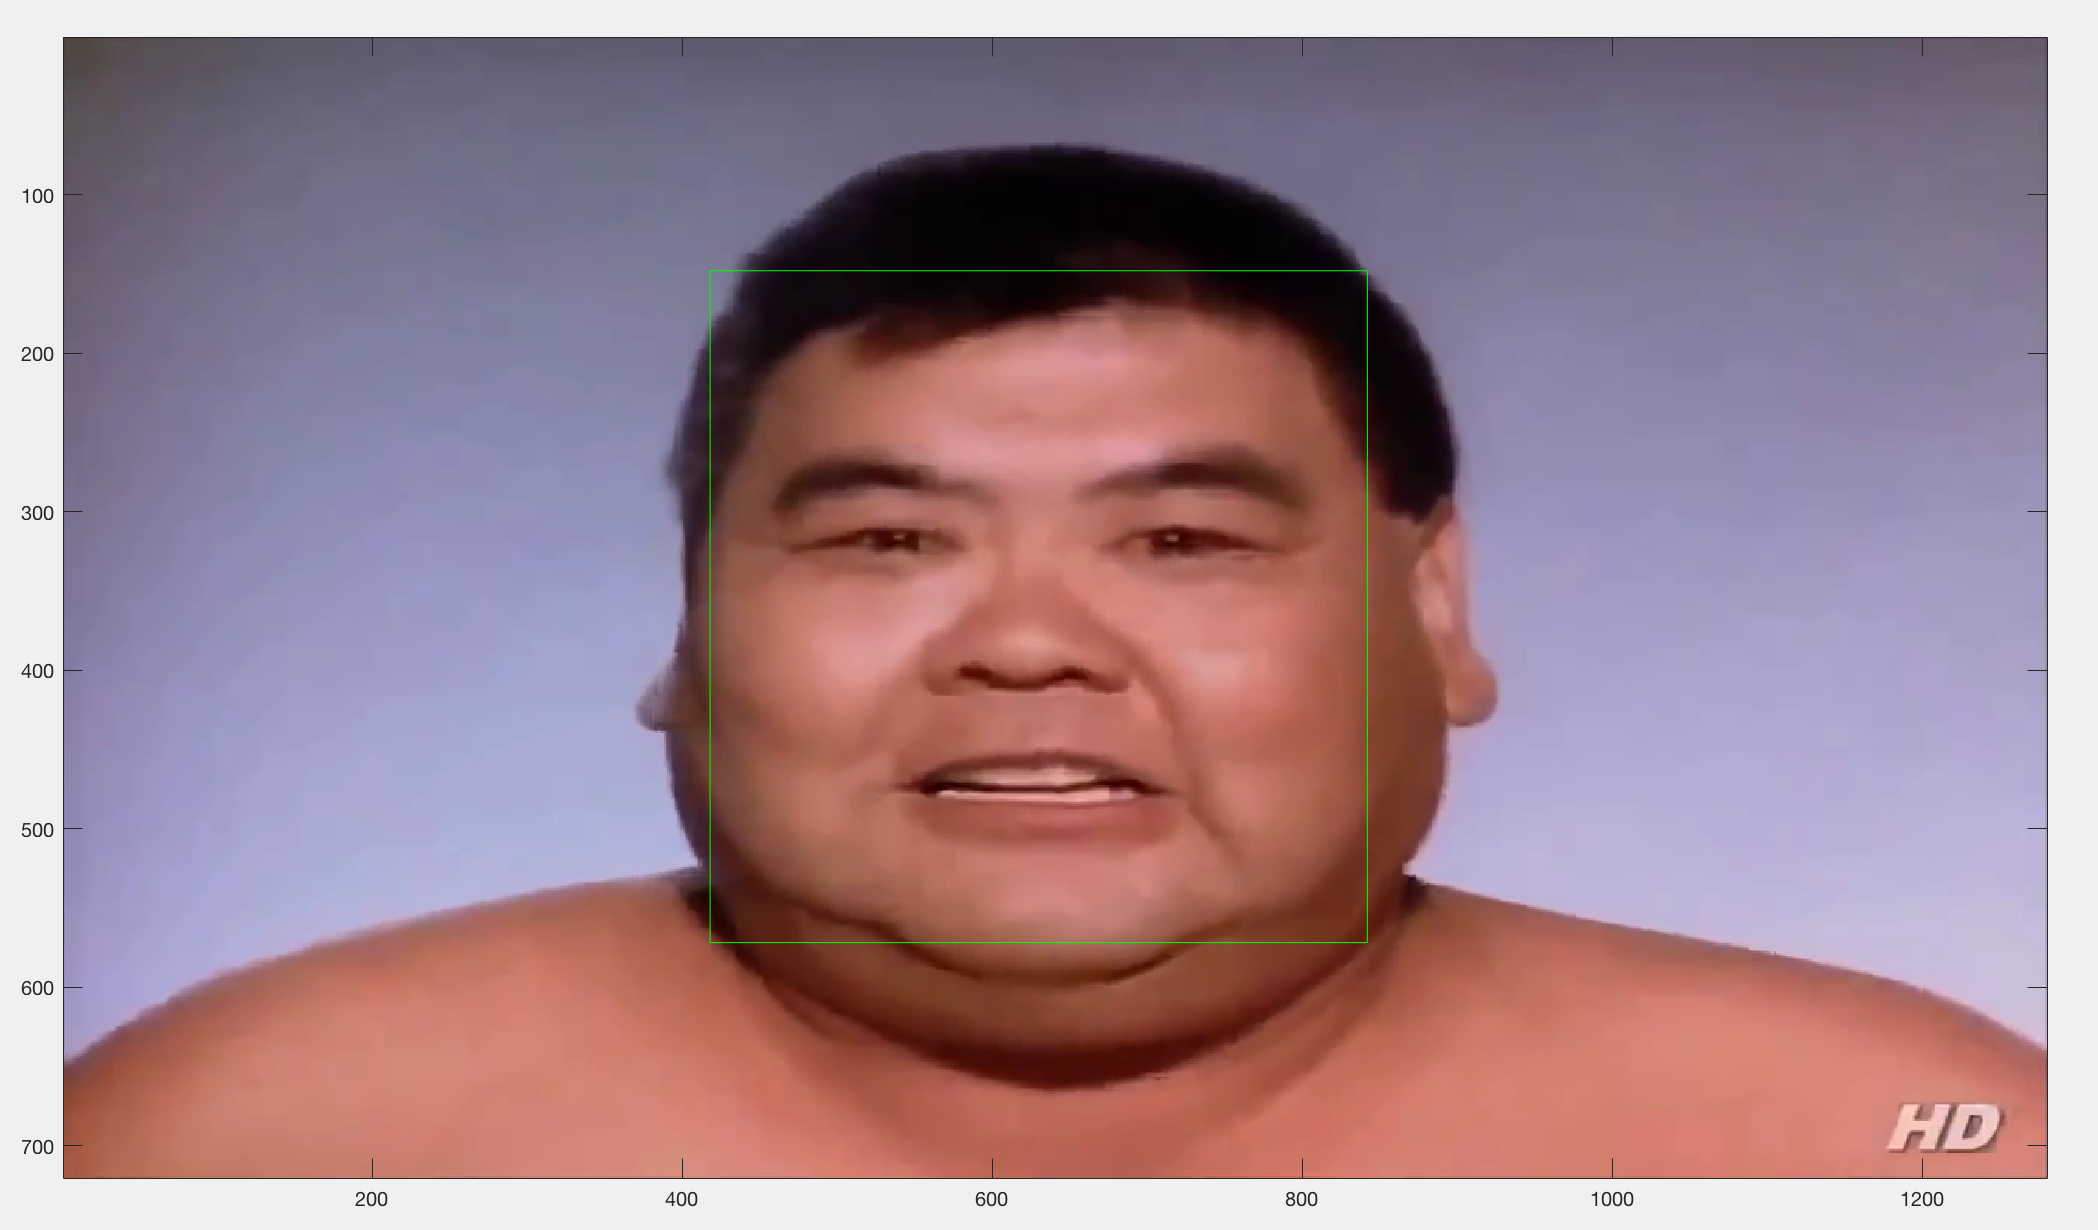
\includegraphics[width=0.6 \textwidth]{./img/ex2/screenshot2.png}
	\caption[The man is looking to the front]{ In this case the man is looking to the front and the face is detected correctly. }
	\label{fig:video2}
\end{figure}

\begin{figure}[h!tb]
	\centering
		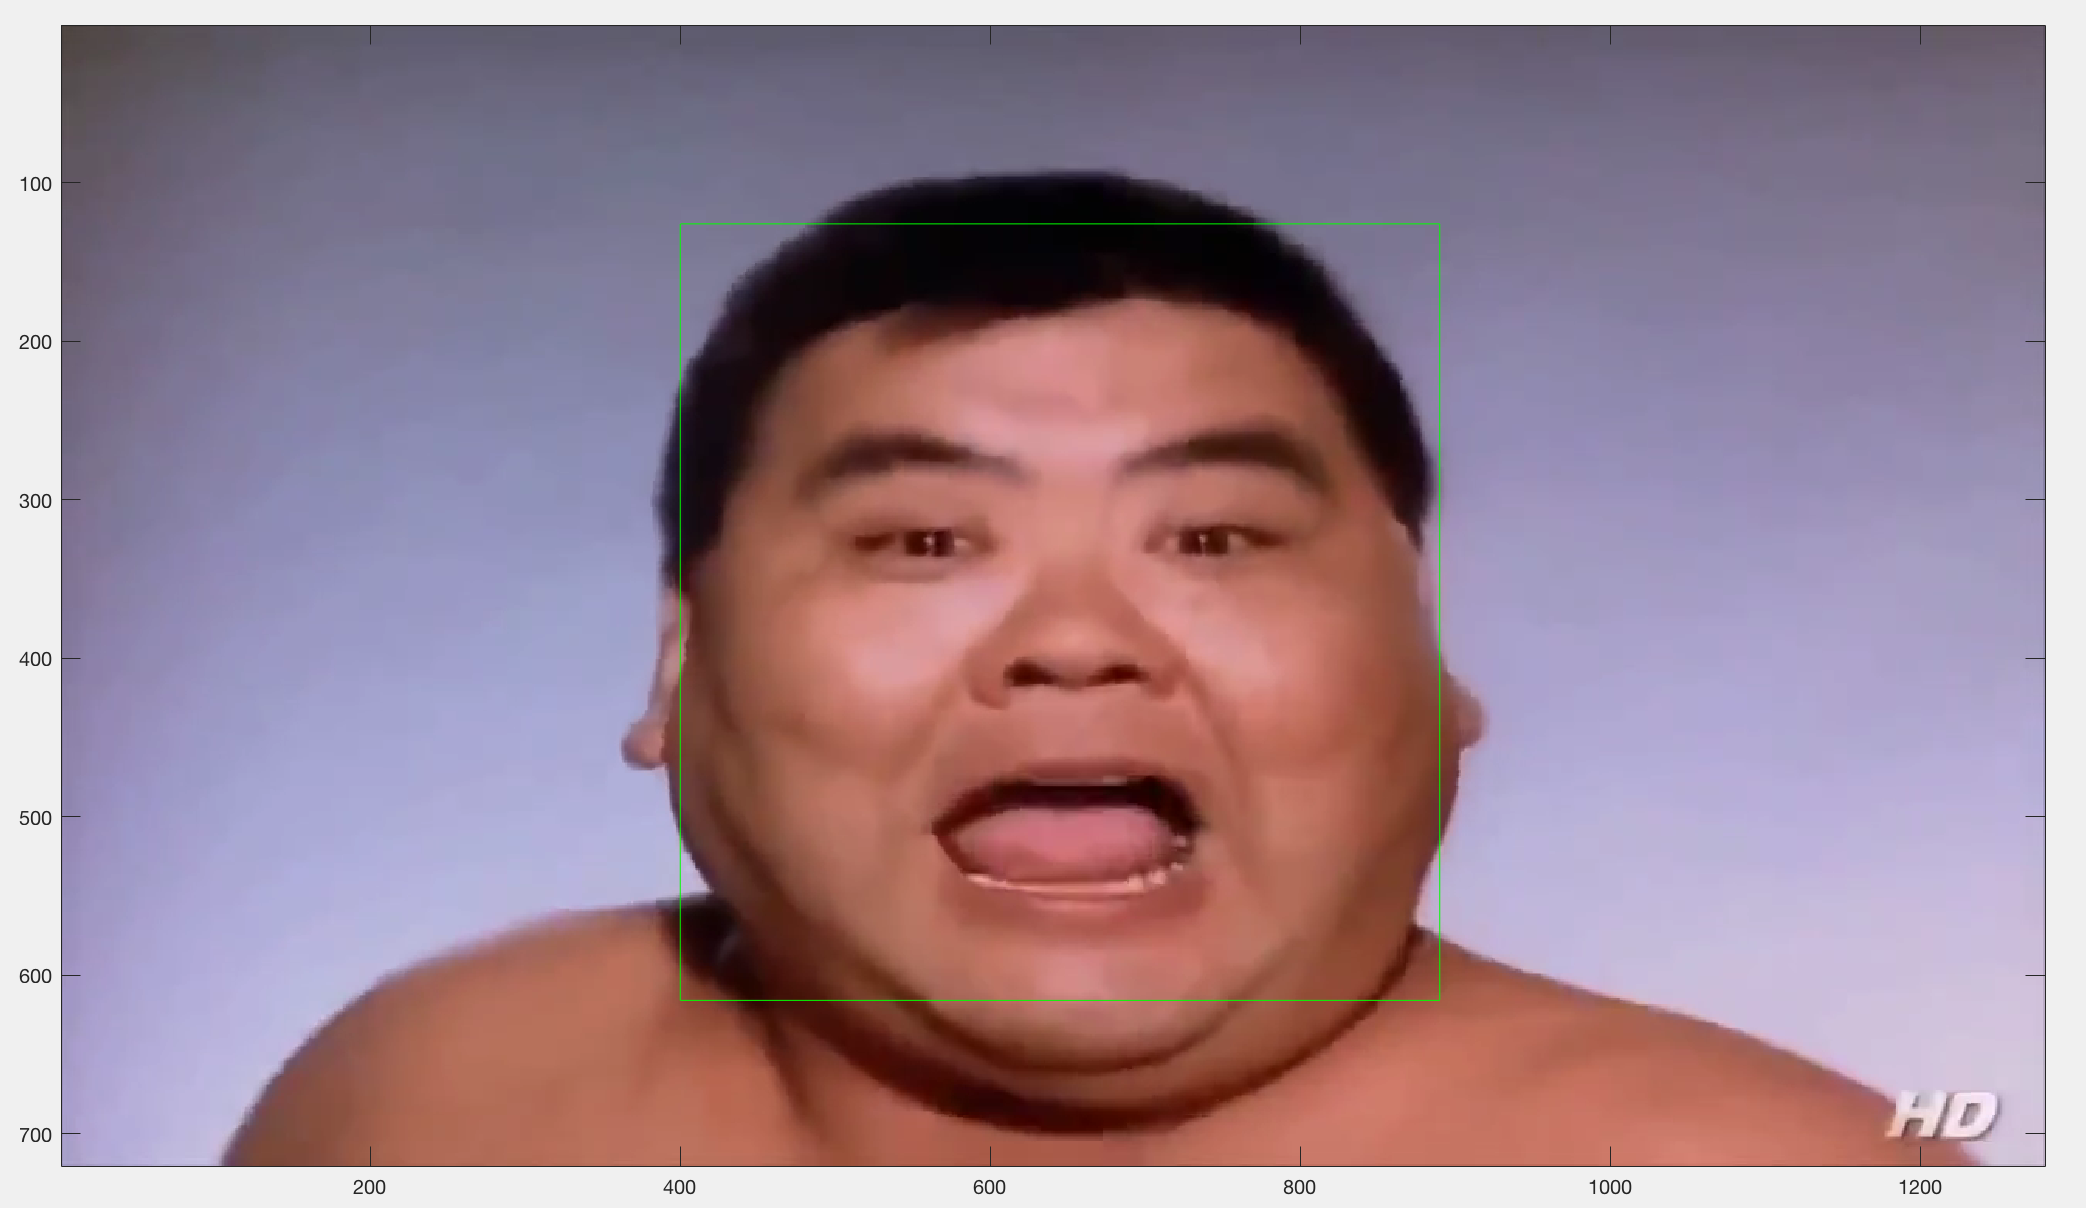
\includegraphics[width=0.6 \textwidth]{./img/ex2/screenshot4.png}
	\caption[The man is looking to the front with his mouth wide open]{ In this case the man is looking to the front with his mouth with open. Even so the Viola \& Jones' features are robust enough to correctly distinguish the face. }
	\label{fig:video4}
\end{figure}

\begin{figure}[h!tb]
	\centering
		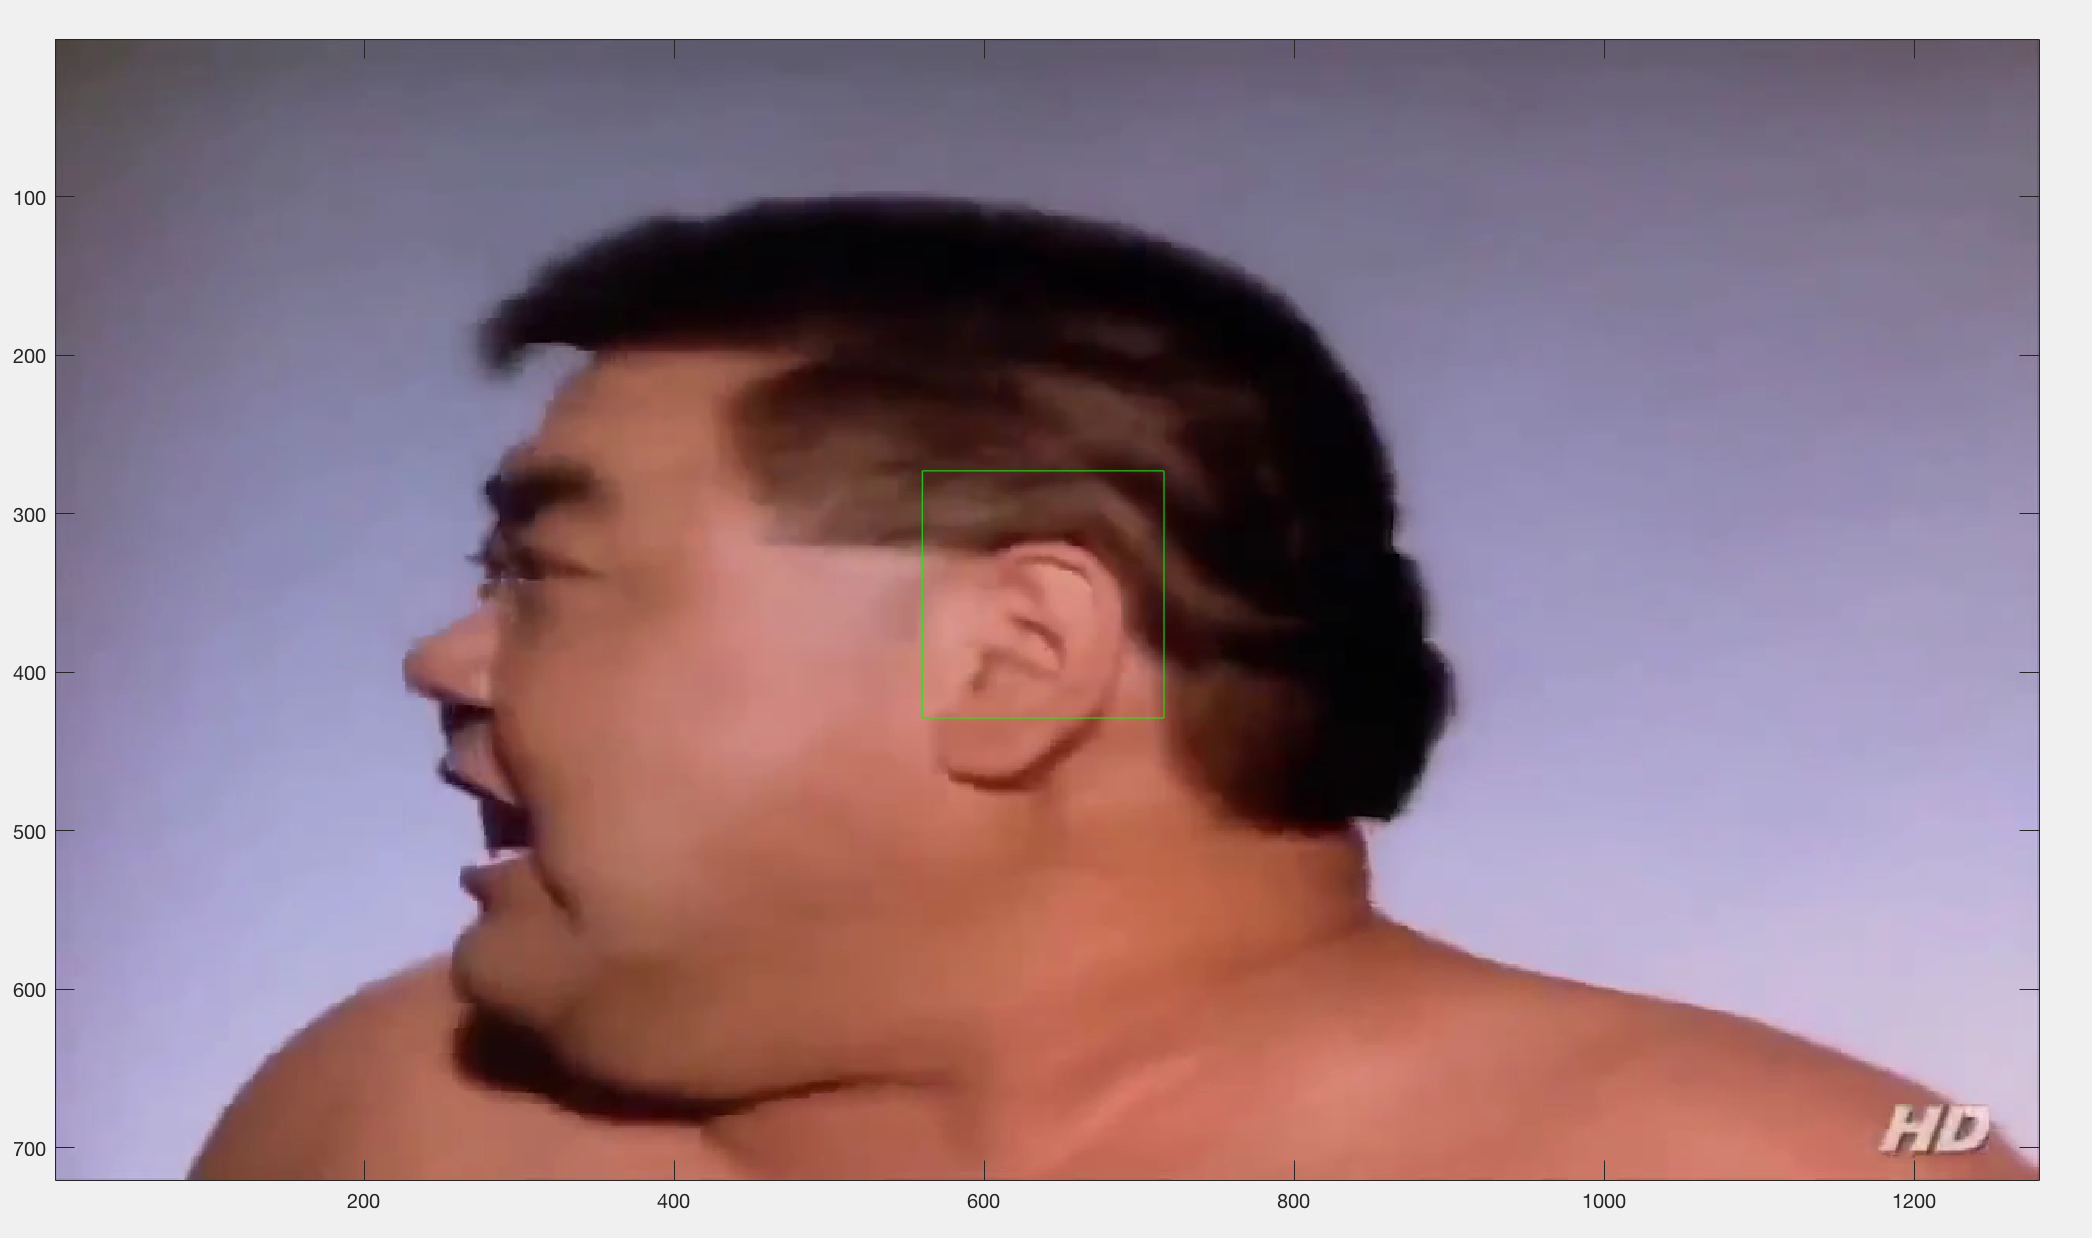
\includegraphics[width=0.6 \textwidth]{./img/ex2/screenshot0.png}
	\caption[Frame from the video in which a man appears with his head turned to the side]{ Frame from the video in which a man appears with his head turned to the side. Notice how his ear is incorrectly detected as a face. }
	\label{fig:video0}
\end{figure}

\begin{figure}[h!tb]
	\centering
		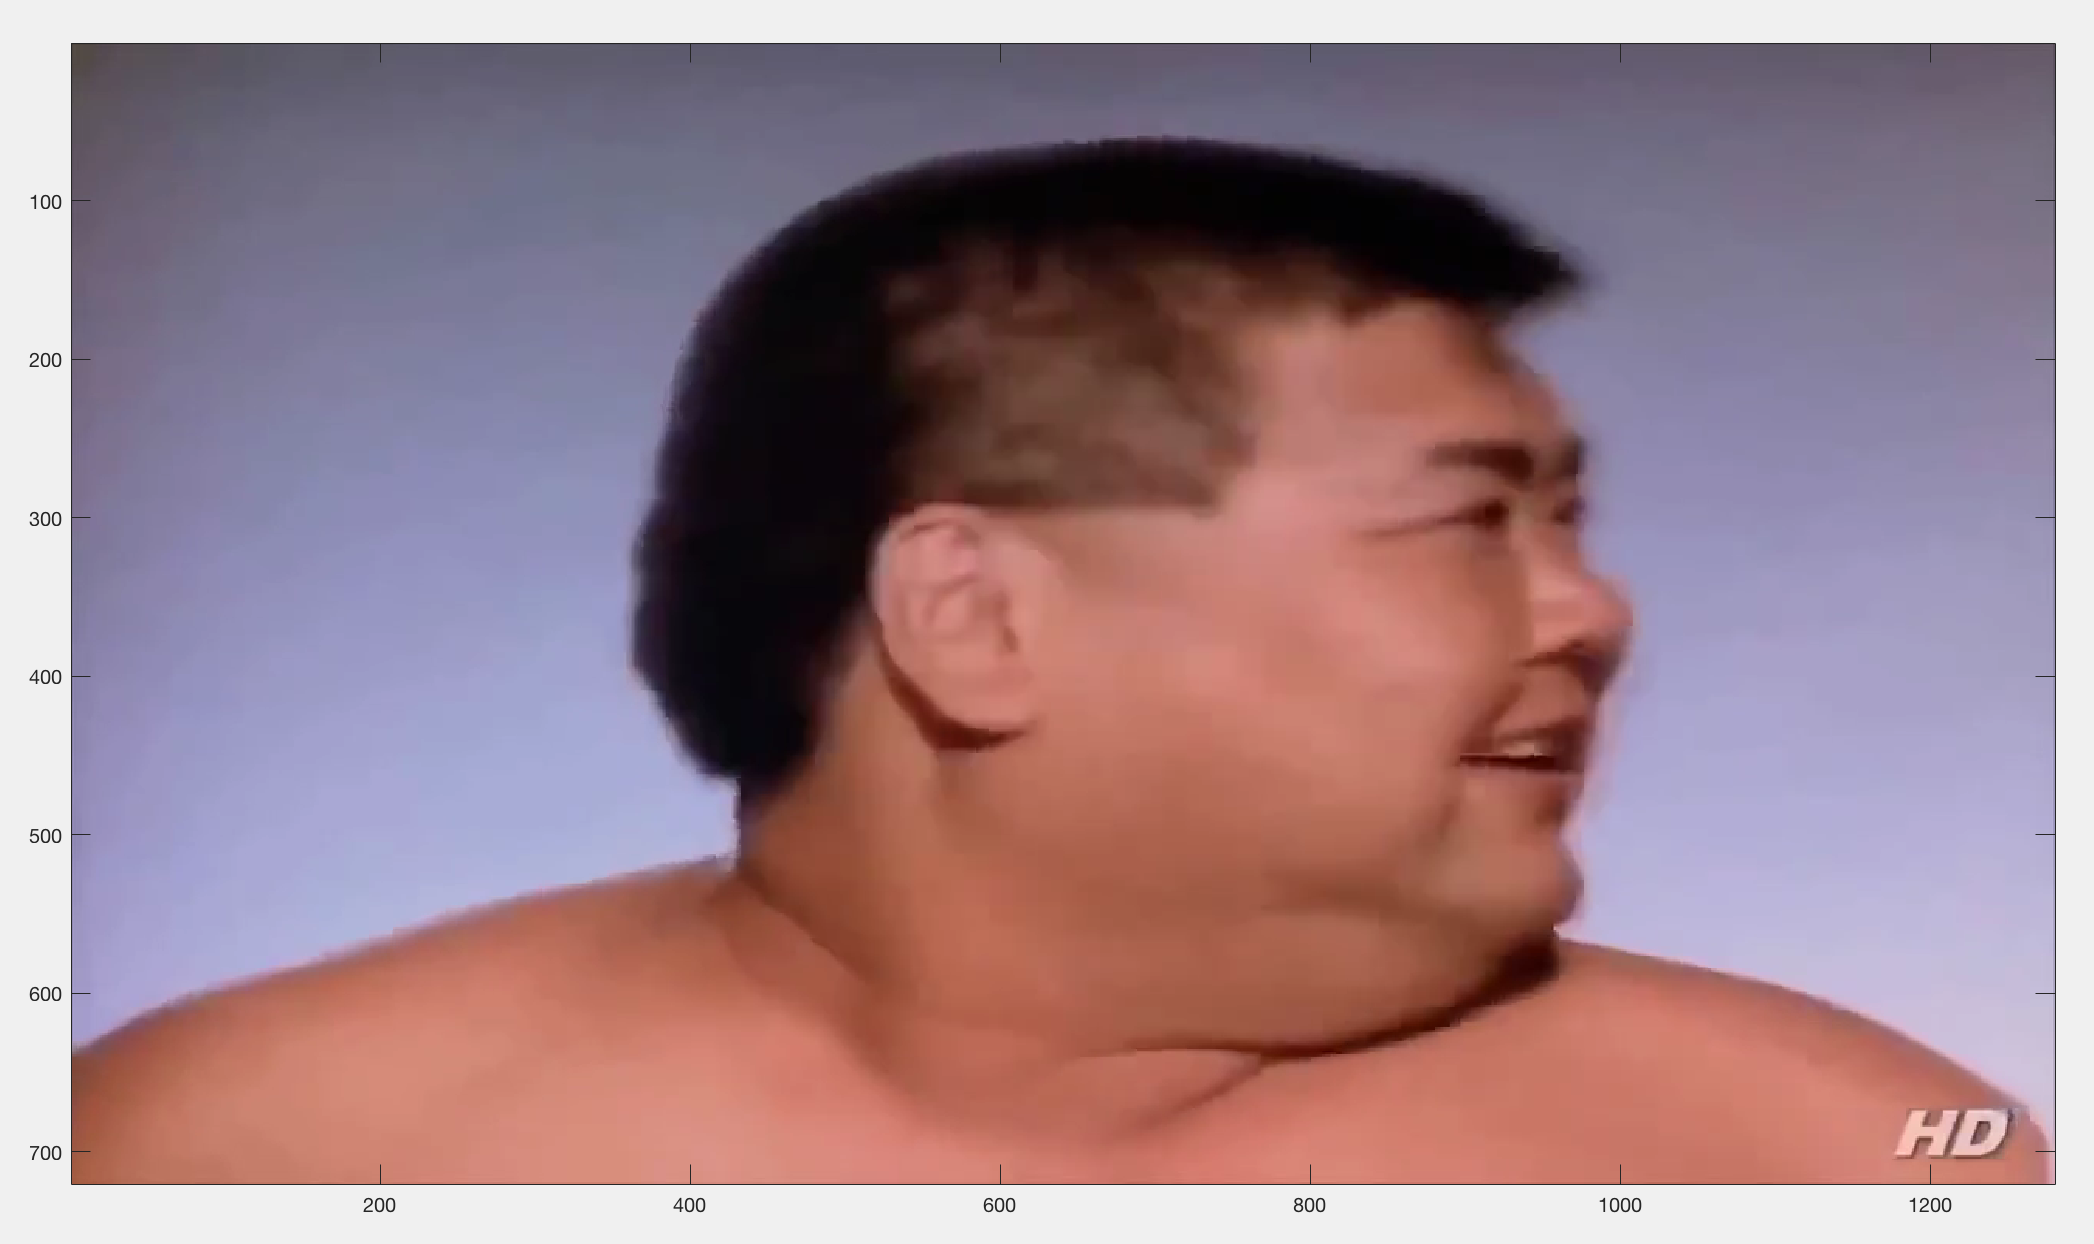
\includegraphics[width=0.6 \textwidth]{./img/ex2/screenshot1.png}
	\caption[The man's head is turned to the other side]{ Frame from the video in which the same man appears with his head turned to the other side. In this case, no face is detected at all (which is preferable than an wrongly detected face). }
	\label{fig:video1}
\end{figure}

\begin{figure}[h!tb]
	\centering
		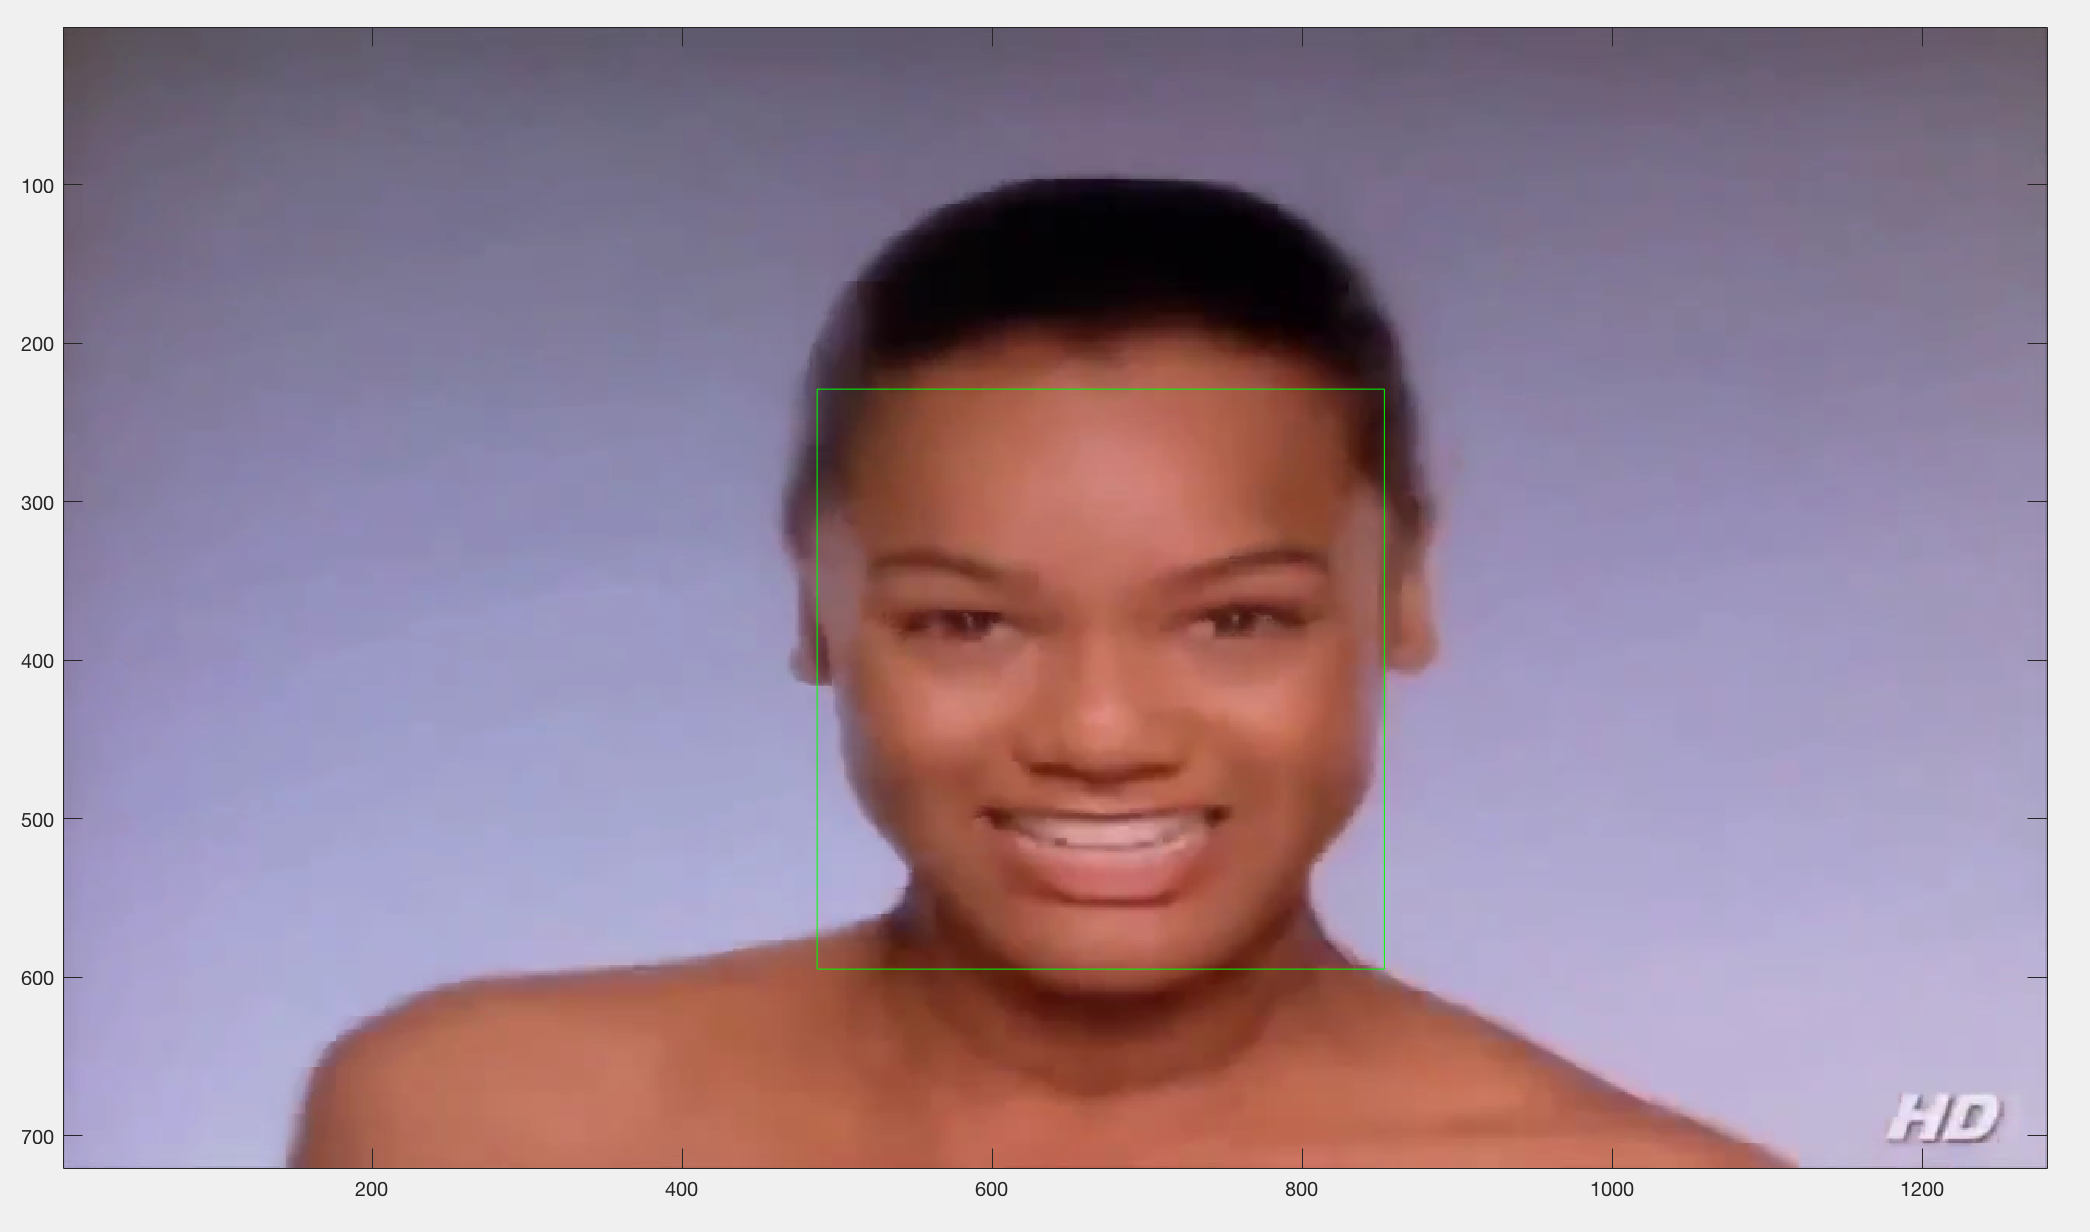
\includegraphics[width=0.6 \textwidth]{./img/ex2/screenshot6.png}
	\caption[Now the detector deals with the face of a woman instead of a man]{ Now the detector is correctly detecting the face of a smiling woman }
	\label{fig:video6}
\end{figure}